%%%%               %%%%
%%%% PLANIFICACIÓN %%%%
%%%%              %%%%

\chapter{Planificación}
\label{chap:planificación}

\lettrine{L}{a} creación de este TFG comparte las características generales de cualquier proyecto, ya que tiene un objetivo concreto y definido, no es una actividad rutinaria, tiene unas fechas de comienzo y de fin. Un proyecto necesita recursos en forma de tiempo, mano de obra, herramientas y conocimiento. En este capítulo se aborda la planificación elaborada.


\section{Recursos necesarios}

Para acometer el proyecto son necesarios varios tipos de recursos:

\begin{itemize}
    \item \textbf{Humanos}
        \begin{itemize}
            \item Un Product Owner, rol asignado al director del proyecto.
            \item Un analista.
            \item Un diseñador.
            \item Un equipo de desarrollo, formado íntegramente por el alumno.
        \end{itemize}
    \item \textbf{Software}: todos los recursos software utilizados son aplicaciones sin coste económico, mucho de ellos, además, software libre.
    \item \textbf{Hardware}: el portátil, pantalla y otros accesorios utilizados.
\end{itemize}

El rol de Product Owner lo realiza el director del proyecto, como se explicó en la Sección \ref{sec:uso-scrum-en-el-proyecto}. Las funciones de análisis, diseño y desarrollo fueron asumidas por el alumno. Cabe destacar que la colaboración para la creación de una interfaz gráfica a este proyecto fue realizada por otro alumno de la Facultad de Informática, no obstante debe quedar claro que no intervino en ningún momento en la elaboración de la parte del trabajo presentada en esta memoria.

\subsection{Planificación económica}

De los recursos utilizados para el proyecto se deducen directamente los costes económicos incurridos. En la Tabla \ref{tab:costes-proyecto} se presentan todos los gastos. Para el cálculo de los costes salariales se consultó el \emph{Convenio colectivo del sector de empresas de ingeniería y oficinas de estudios técnicos} en su página del BOE \footnote{\url{https://www.boe.es/diario_boe/txt.php?id=BOE-A-2019-14977}}.

\begin{table}[ht]
    \centering
    \begin{tabular}{l l l l}
        Recurso & Coste (€/h) & Tiempo (h) & Coste total (€) \\
        \hline
        \hline
        Jefe de proyecto & 42 & x & x \\
        Analista & 35 & x & x \\
        Diseñador & 35 & x & x \\
        Programador & 30 & x & x \\
        Equipamiento informático & -- & x & 900 \\
        Microsoft Project (licencia universitaria) & -- & - & 0 \\
		Otro software & -- & - & 0 \\    
        \hline
        \hline
        TOTAL & & - & x \\        
    \end{tabular}
	\caption{Costes del proyecto.}    
	\label{tab:costes-proyecto}
\end{table}

\section{Planificación temporal inicial}

En la Imagen \ref{fig:gantt-inicial} se presenta el diagrama de Gantt inicial de la planificación con el desglose de tareas. Una de las dificultades para la planificación consistió en no saber en qué momento del proyecto sería necesario abordar la integración con la interfaz web. Inicialmente se asumió que ocurriría con posterioridad al trabajo de desarrollo y antes de comenzar la escritura de la memoria. En este plan inicial se contemplaban 524 horas de trabajo.

\begin{figure}[hp!]
    \centering
    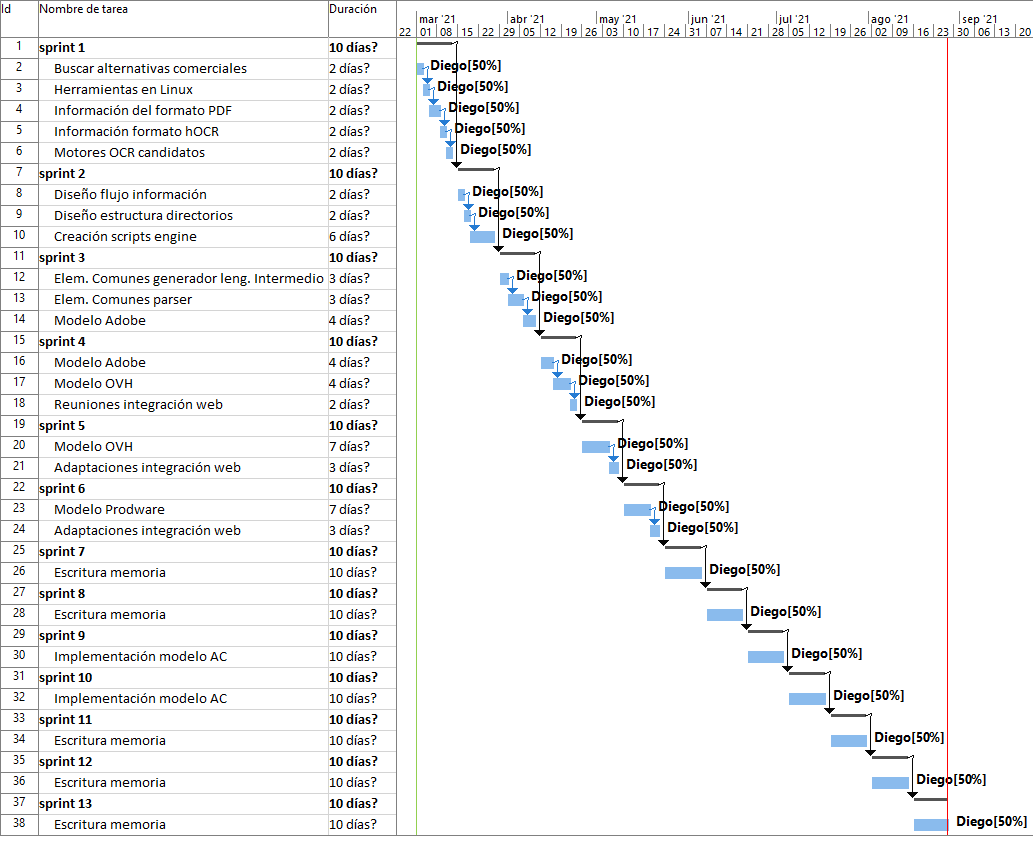
\includegraphics[angle=90,width=1.0\textwidth]{imaxes/f-planificacion/gantt-inicial.png}
    \caption{Diagrama de Gantt y tareas iniciales del proyecto.}
    \label{fig:gantt-inicial}
\end{figure}

\section{Sprints}

Se expone a continuación la distribución del trabajo a lo largo de los sprints. Por motivos de compatibilidad con el trabajo y responsabilidades personales, se escogió una fórmula de 20 horas de trabajo semanal y una duración de cada sprint de 2 semanas.

\subsection{Sprint 1}

Este primer sprint consistió por completo en un spike con el objetivo de recabar toda la información necesaria para plantear el proyecto a nivel técnico. Algunos de los aspectos sobre los que se adquirió conocimiento fueron:

\begin{itemize}
    \item Alternativas comerciales en la misma temática.
    \item Herramientas y librerías disponibles en Linux para manipular PDF.
    \item Funcionamiento del formato PDF a nivel interno.
    \item Formatos de salida de los motores de OCR, es especial del seleccionado, hOCR.
    \item Posibles engines de OCR candidatos para el proyecto
\end{itemize}

\subsection{Sprint 2}

Con el conocimiento de reunido se procedió a la construcción inicial del sistema para el procesamiento por lotes de los trabajos. Además de diseñar la estructura de directorios utilizada por el proyecto, se crearon el Makefile general, utilizado para las compilaciones y los scripts para implementar el motor.

\subsection{Sprint 3}

En el sprint 3 se crearon las implementaciones iniciales del generador de lenguaje intermedio y se preparó el primer parser, que se probó con los documentos de Adobe. Para la construcción de los parsers se deseaba un enfoque modular, que no es habitual en este tipo de herramientas. El objetivo era tener un único programa ejecutable para el parser y un conjunto de plugins que implementarían cada uno un modelo de documento. Dado que este no es el tipo de configuración más habitual, llevó un poco más de tiempo que otros planteamientos más sencillos.

\subsection{Sprint 4}

En este sprint se añadió soporte para la generación de código intermedio y parsing del modelo de OVH. También tuvieron lugar las primeras reuniones de trabajo para explicar el proyecto y decidir las adaptaciones necesarias de cara al prototipo.

\subsection{Sprint 5}

Se completó el modelo de documento del proveedor Prodware. Además se abordaron de forma paralela las tareas relacionadas con el prototipo web. Hubo varias reuniones para facilitar la implementación de aspectos que no habían sido considerados, como  la necesidad de generar imágenes de las páginas individuales de cada documento, cambio del formato de la marca de tiempo para mejorar la compatibilidad entre sistemas de ficheros y la dockerización de la aplicación.

\subsection{Sprints 6, 7 y 8}

En estas tres semanas se abordó la escritura inicial de la memoria, con la previsión de dejar tiempo al final del proyecto para completarla.

\subsection{Sprint 9}

Implementación de los modelos basados en imagen.

\subsection{Sprint 10}

Implementación de los modelos basados en imagen.

\subsection{Sprint 11}

El sprint 11 se utilizó para construir el prototipo del editor de coordenadas.

\subsection{Sprint 12 y 13}

Los últimos dos sprints se dedicaron a finalizar la escritura de la memoria.


\section{Planificación temporal final}

% TODO explicar que las reuniones se adelantaron a las fechas previstas
